%% LyX 2.4.3 created this file.  For more info, see https://www.lyx.org/.
%% Do not edit unless you really know what you are doing.
\documentclass{beamer}
\usepackage{mathpazo}
\usepackage[latin9]{inputenc}
\setcounter{secnumdepth}{3}
\setcounter{tocdepth}{3}
\usepackage{array}
\usepackage{multirow}
\usepackage{amstext}
\usepackage{amssymb}
\usepackage{graphicx}
\ifx\hypersetup\undefined
  \AtBeginDocument{%
    \hypersetup{bookmarks=false,
 breaklinks=false,pdfborder={0 0 1},backref=section,colorlinks=false}
  }
\else
  \hypersetup{bookmarks=false,
 breaklinks=false,pdfborder={0 0 1},backref=section,colorlinks=false}
\fi

\makeatletter

%%%%%%%%%%%%%%%%%%%%%%%%%%%%%% LyX specific LaTeX commands.
%% Because html converters don't know tabularnewline
\providecommand{\tabularnewline}{\\}

%%%%%%%%%%%%%%%%%%%%%%%%%%%%%% Textclass specific LaTeX commands.
% this default might be overridden by plain title style
\newcommand\makebeamertitle{\frame{\maketitle}}%
% (ERT) argument for the TOC
\AtBeginDocument{%
  \let\origtableofcontents=\tableofcontents
  \def\tableofcontents{\@ifnextchar[{\origtableofcontents}{\gobbletableofcontents}}
  \def\gobbletableofcontents#1{\origtableofcontents}
}

%%%%%%%%%%%%%%%%%%%%%%%%%%%%%% User specified LaTeX commands.
%\newtheorem{theorem}{Theorem}
%\newtheorem{corollary}[theorem]{Corollary}
%\newtheorem{definition}[theorem]{Definition}
%\newtheorem{example}[theorem]{Example}
%\newtheorem{lemma}[theorem]{Lemma}
%\newtheorem{problem}[theorem]{Problem}
%\newtheorem{solution}[theorem]{Solution}


%%%%%%%%%%%%%%%%%%%%%%%%%%%%%%%%%%%%%%%%%%%%%%%%%%%%%%%%%%%%%%%%%%%%%%%%%%%%%%%%%%%%%%%%%%%%%%%%%%%%%%%%%%%%%%%%%%%%%%%%%%%%%%%%%%%%%%%%%%%%%%%%%%%%%%%%%%%%%%%%%%%%%%%%%%%%%%%%%%%%%%%%%%%%%%%%%%%%%%%%%%%%%%%%%%%%%%%%%%%%%%%%%%%%%%%%%%%%%%%%%%%%%%%%%%%%
\usepackage{graphicx}
\usepackage{amsfonts}
\usepackage{multimedia}
\usepackage{pstricks}
%\usepackage{pst-plot}
\usepackage{xcolor}
\beamertemplatenavigationsymbolsempty
\date{} 
\setbeamertemplate{footline}[frame number]

\setcounter{MaxMatrixCols}{10}
%TCIDATA{OutputFilter=LATEX.DLL}
%TCIDATA{Version=5.50.0.2953}
%TCIDATA{<META NAME="SaveForMode" CONTENT="2">}
%TCIDATA{BibliographyScheme=Manual}
%TCIDATA{Created=Friday, October 09, 2009 16:36:30}
%TCIDATA{LastRevised=Monday, April 01, 2013 11:48:45}
%TCIDATA{<META NAME="GraphicsSave" CONTENT="32">}
%TCIDATA{<META NAME="DocumentShell" CONTENT="Other Documents\SW\Slides - Beamer">}
%TCIDATA{CSTFile=beamer.cst}

\newtheorem{acknowledgement}[theorem]{Acknowledgement}\newtheorem{algorithm}[theorem]{Algorithm}\newtheorem{axiom}[theorem]{Axiom}\newtheorem{case}[theorem]{Case}\newtheorem{claim}[theorem]{Claim}\newtheorem{conclusion}[theorem]{Conclusion}\newtheorem{condition}[theorem]{Condition}\newtheorem{conjecture}[theorem]{Conjecture}\newtheorem{criterion}[theorem]{Criterion}\newtheorem{exercise}[theorem]{Exercise}\newtheorem{notation}[theorem]{Notation}\newtheorem{proposition}[theorem]{Proposition}\newtheorem{remark}[theorem]{Remark}\newtheorem{summary}[theorem]{Summary}\newtheorem{prediction}{Prediction}\setbeamertemplate{itemize items}[circle]
\setbeamercolor{itemize item}{fg= black}
\setbeamercolor{itemize subitem}{fg=black}
\setbeamercolor{itemize subsubitem}{fg= black}
\setbeamercolor{frametitle}{fg=purple}
\setbeamercolor{title}{fg=black}
\setbeamercolor{caption name}{fg=black}


%
\usefonttheme{serif}
\setbeamersize{text margin left=5pt,text margin right=5pt}
%%\usetheme{Singapore}
\usetheme{default}
%%\input{tcilatex}
%\useoutertheme{miniframes}
%\hypersetup{colorlinks=true,linkcolor=white}
%%\setbeamertemplate{footline}[frame number]
%\beamertemplatenavigationsymbolsempty
%%\setbeamertemplate{footline}{\hspace*{.5cm}\scriptsize{\insertauthor\hspace*{40pt}\insertframenumber}}

%\begin{document}

\makeatother

\begin{document}
\title{{\Large\textrm{\textsc{\textcolor{violet}{AI and Human Capital Accumulation:
Aggregate and Distributional Implications}}}}{\LARGE\textrm{\textcolor{violet}{\medskip{}
}}}}
\author{{\large$\begin{array}{cccc}
\text{Yang K. Lu} &  &  & \text{\text{\textbf{Eunseong Ma}}}\\
\text{HKUST} &  &  & \text{Yonsei}
\end{array}$}~\\
\vspace{0.6cm}
~\\
{\large\color{blue}KDI}}
\date{{\normalsize\textrm{May 21, 2026}}}

\makebeamertitle

\begin{frame}{Introduction{\small\textbf{\textit{\textcolor{brown}{~~Motivation}}}}}

\begin{itemize}
\item AI is reshaping labor markets in ways that are both profound and uneven
{\small\textit{\textcolor{gray}{(Revelio Labs, 2025; Souza, 2025;
Asam and Heller, 2025)}}}.
\end{itemize}
\medskip{}

\begin{itemize}
\item However, workers can respond by re-optimizing their \textcolor{blue}{human
capital investments.}
\begin{itemize}
\item Confidence in traditional higher education is eroding while demand
for AI reskilling is surging {\small\textit{\textcolor{gray}{(Public
Agenda, 2022;10 Oliver Wyman Forum, 2024)}}}{\small\par}
\end{itemize}
\item \textit{\textcolor{brown}{Yet most studies abstract from these endogenous
human-capital responses.}}
\end{itemize}
\medskip{}

\begin{itemize}
\item This paper addresses this gap by examining 
\begin{itemize}
\item \textcolor{red}{how AI-driven changes affects human capital investment,}
\item \textcolor{red}{how these adjustments reshape aggregate and distributional
outcomes.}
\end{itemize}
\end{itemize}
\end{frame}

\begin{frame}{What We Do}

\begin{itemize}
\item We construct a model with human capital investment and a sectoral
structure.

\medskip{}

\item \textbf{Market Incompleteness}
\begin{itemize}
\item Households differ in assets, human capital, and idiosyncratic labor
productivity.
\item They make an indivisible labor-supply choice and a standard savings
decision.
\end{itemize}
\medskip{}

\item \textbf{\textcolor{red}{Human Capital Investment}}
\begin{itemize}
\item On-the-job learning vs. full-time learning
\item Segmented sectors based on HC
\end{itemize}
\medskip{}

\item \textbf{\textcolor{brown}{Key Channel:}}\textcolor{brown}{{} }\textbf{\textcolor{brown}{Rich
interactions among HC investment, labor supply, and saving decisions.}}
\end{itemize}
\end{frame}

\begin{frame}{What We Do}

\medskip{}

\begin{itemize}
\item \textbf{Assumption for AI Adoption}
\begin{itemize}
\item Common assumption: It is anticipated
\end{itemize}
\begin{enumerate}
\item \textbf{\textcolor{blue}{Baseline experiment:}} an shock that raises
productivity in the low and high sectors
\item \textbf{\textcolor{brown}{AI+ experiment:}}\textcolor{brown}{{} }raises
the HC threshold for high-sector entry
\end{enumerate}
\end{itemize}
\medskip{}

\begin{itemize}
\item \textbf{Methodological Approach}
\begin{enumerate}
\item A two-period version of the model
\begin{itemize}
\item to see analytical results that isolate the core mechanisms.
\end{itemize}
\item A full dynamic quantitative model 
\begin{itemize}
\item to incorporate transition dynamics and general equilibrium effects,
\item to quantify i) direct and indirect effect of AI and ii) aggregate
and distributional outcomes.
\end{itemize}
\end{enumerate}
\end{itemize}
\end{frame}

\begin{frame}{What We Find}

\medskip{}

\begin{enumerate}
\item \textbf{Analytical Results}
\begin{itemize}
\item An anticipated AI shock generates endogenous divergence in HC investment
incentives. 
\item In the AI+ case, a\textbf{ churning effect} additionally emerges near
the new high-sector cutoff.
\end{itemize}
\medskip{}

\item \textbf{Quantitative Results}
\begin{enumerate}
\item \textbf{Aggregate Effect }
\begin{itemize}
\item AI shock generates\textbf{ voluntary job polarization}
\item GDP and consumption rise, while aggregate employment falls. 
\item Endogenous HC adjustment amplifies the effects through more efficient
sectoral reallocation.
\item In the AI+ experiment, it becomes more important due to the \textbf{churning
effect. }
\end{itemize}
\item \textbf{\textcolor{black}{Distributional Effects}}
\begin{itemize}
\item Income and earnings inequality rises due to the polarization.
\item Wealth inequality changes little in the baseline but rises in the
AI+ experiment.
\end{itemize}
\end{enumerate}
\end{enumerate}
\end{frame}

\begin{frame}{Related Literature}

\begin{itemize}
\item \textbf{\textcolor{black}{Technological advancements on job polarization}}
\begin{itemize}
\item \textit{\textcolor{gray}{Goos and Manning (2007), Autor and Dorn (2013),
Goos et al. (2014), Acemoglu and Restrepo (2020)}}
\end{itemize}
\smallskip{}

\item \textbf{\textcolor{black}{Automation increases human capital investment:}}
\begin{itemize}
\item \textit{\textcolor{gray}{Atkin (2016), Beaudry et al. (2016), Dauth
et al. (2021), Di Giacomo and Lerch (2023)}}
\end{itemize}
\smallskip{}

\item \textbf{\textcolor{black}{Automation exacerbates wealth inequality}}
\begin{itemize}
\item \textit{\textcolor{gray}{Sachs and Kotlikoff (2012), Prettner and
Strulik (2020)}}
\end{itemize}
\end{itemize}
\smallskip{}

\begin{itemize}
\item \textbf{\textcolor{purple}{Our Contributions: analyzing effects of
AI on both aggregate and distributional outcomes, highlighting }}
\begin{itemize}
\item \textbf{\textcolor{purple}{i) the roles of human capital adjustment, }}
\item \textbf{\textcolor{purple}{ii) general equilibrium feedback, and }}
\item \textbf{\textcolor{purple}{iii) transition dynamics.}}
\end{itemize}
\end{itemize}
\end{frame}


\section{Model}
\begin{frame}{~}

\begin{center}
{\huge\textbf{Model Environment}}{\huge\par}
\par\end{center}

\end{frame}

\begin{frame}{Households{\small\textbf{\textit{\textcolor{brown}{~~Heterogeneity}}}}}

\begin{itemize}
\item \textcolor{blue}{Idiosyncratic shocks:} Households face idiosyncratic
labor-productivity and learning-ability shocks, $z$ and $y$, which
follow AR(1) process in logs: 
\end{itemize}
\medskip{}

\begin{center}
$\log z'=\rho_{z}\log z+\varepsilon_{z},\,\,\,\,\varepsilon_{z}\stackrel{iid}{\sim}\mathcal{N}(0,{\sigma_{z}}^{2})$.
\par\end{center}

\medskip{}

\begin{center}
$\log y'=\rho_{y}\log y+\varepsilon_{y},\,\,\,\,\varepsilon_{y}\stackrel{iid}{\sim}\mathcal{N}(0,{\sigma_{y}}^{2})$.
\par\end{center}
\begin{itemize}
\item \textcolor{blue}{Incomplete asset market:} Households cannot issue
any assets contingent on their future idiosyncratic risks.
\end{itemize}
\end{frame}

\begin{frame}{Households{\small\textbf{\textit{\textcolor{brown}{~~Human capital}}}}}

\begin{itemize}
\item Human capital investment can take three levels of effort: $\{0,e_{L},e_{H}\}$. 
\item A non-working HH is free to choose any of the effort levels but a
working HH cannot devote $e_{H}$: 
\end{itemize}
\begin{equation}
e_{t}\in\left\{ \begin{array}{cl}
\{0,e_{L}\} & \text{ if }n>0\\
\{0,e_{L},e_{H}\} & \text{ if }n=0
\end{array}\right.\label{eq:x-1}
\end{equation}

\medskip{}

\begin{itemize}
\item Its contribution to next-period human capital is subject to the productivity
shock: 
\begin{equation}
h_{t+1}=y_{t}e_{t}+(1-\delta)h_{t}
\end{equation}
\item Sectoral productivity for effective labor units 
\begin{equation}
x(h)=\left\{ \begin{array}{cl}
1-\lambda & \text{low sector if }h<h_{M}\\
1 & \text{middle sector if }h_{M}\leq h<h_{H}\\
1+\lambda & \text{high sector if }h\geq h_{H}
\end{array}\right.\label{eq:x}
\end{equation}
\end{itemize}
\end{frame}

\begin{frame}{Households{\small\textbf{\textit{\textcolor{brown}{~~Problem}}}} }

\begin{itemize}
\item A household maximizes her expected lifetime utility consumption, $c_{t},$
and hours of work, $h_{t}:$ 

\medskip{}

\begin{equation}
\max_{\left\{ c_{t},a_{t+1},n_{t},e_{t}\right\} _{t=0}^{\infty}}E_{0}\left[\sum\limits_{t=0}^{\infty}\beta^{t}(\ln c_{t}-\chi_{n}n_{t}-\chi_{e}e_{t})\right]\text{ s.t.}
\end{equation}
\textcolor{black}{
\begin{align}
c_{t}+a_{t+1} & =w_{t}{\color{blue}{\color{black}z_{t}n_{t}x(h_{t})+(1+r_{t})a_{t}}}
\end{align}
}
\[
a_{t+1}\ge0.
\]

\item Labor supply is indivisible: $n_{t}\in\{0,\overline{n}\}$.
\end{itemize}
\end{frame}

\begin{frame}{Production technology}

\begin{itemize}
\item Produce output according to Cobb-Douglass production function: 

\begin{equation}
F(K,L)=K^{1-\alpha}L^{\alpha},
\end{equation}
\begin{equation}
K={\textstyle \int a_{i}di,\quad L={\textstyle \int n_{i}z_{i}x(h_{i})di}}
\end{equation}

\end{itemize}
\end{frame}

\begin{frame}{AI Shock}

\begin{itemize}
\item \textbf{Baseline:} AI changes skill premium through $\gamma$ {\small\textit{\textcolor{gray}{(Autor
and Dorn, 2013; Goos et al.,20145)}}}{\small\par}

\begin{equation}
x(h)=\left\{ \begin{array}{cl}
1-\lambda+\gamma\lambda & \text{low sector if }h<h_{M}\\
1 & \text{middle sector if }h_{M}\leq h<h_{H}\\
1+\lambda+\gamma\lambda & \text{high sector if }h\geq h_{H}
\end{array}\right.\label{eq:xAI-1}
\end{equation}

\medskip{}

\item \textbf{AI+ experiment:} AI raises the bar for high-sector entry {\small\textit{\textcolor{gray}{(Bloomberg,
2025)}}}{\small\par}

\begin{equation}
x^{AI+}(h')=\left\{ \begin{array}{cl}
1-\lambda+\gamma\lambda & \text{low sector if }h'<h_{M}\\
1 & \text{middle sector if }h_{M}\leq h'<h'_{H}\\
1+\lambda+\gamma\lambda & \text{high sector if }h'\geq h'_{H}
\end{array}\right.\label{eq:xAI-1-1}
\end{equation}

\end{itemize}
\end{frame}


\section{Model}
\begin{frame}{~}

\begin{center}
{\huge\textbf{Household Decisions in Two-Period Model}}{\huge\par}
\par\end{center}

\end{frame}

\begin{frame}{Assumptions}

\begin{itemize}
\item Period 2 : Households choose labor supply only and consume all. 
\item Period 1 : Households choose labor supply, consumption, saving and
human capital investment. 
\end{itemize}
\bigskip{}

\begin{itemize}
\item We partition households into three ranges:
\end{itemize}
\begin{equation}
h=\left\{ \begin{array}{cl}
[0,h_{M}(1-\delta)^{-1}) & \text{low sector}\\{}
[h_{M}(1-\delta)^{-1},h_{H}(1-\delta)^{-1}) & \text{middle sector}\\{}
[h_{H}(1-\delta)^{-1},h_{\max}] & \text{high sector }
\end{array}\right.\label{eq:xAI-1-1-1}
\end{equation}

\end{frame}

\begin{frame}{Decision Rule}

\begin{center}
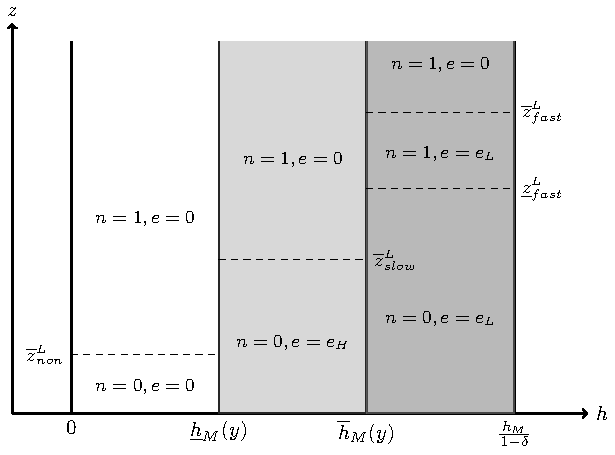
\includegraphics[scale=1]{../figure_204040calib/Figure1.pdf}
\par\end{center}

\end{frame}

\begin{frame}{Key Propositions}

\begin{itemize}
\item HC investment changes savings ultimately depends on the size of two
channels
\begin{enumerate}
\item the crowd-out effect via higher expected future income
\item the precautionary crowd-in effect via heightened future income risk
\end{enumerate}
\medskip{}

\item \textbf{Proposition 1}\textit{ }
\begin{itemize}
\item \textit{HC investment crowds out saving for low-income households
and crowds in saving for high-income households}
\item {\small\textit{Part-time: for $x<x^{\ast}(a,t)$, $e=e_{L}$ lowers
saving $\Delta(x,a;t>1)<0$; for $x>x^{\ast}(a,t)$, $e=e_{L}$ raises
saving $\Delta(x,a;t>1)>0$.}}{\small\par}
\item {\small\textit{Full-time: for $x<\min\{x^{*}(a,t),\hat{x}(a,t)\}$,
$e=e_{H}$ lowers saving $\Delta_{\text{full-time}}(x,a;t>1)<0$;
for $x>\max\{x^{*}(a,t),\hat{x}(a,t)\}$, $e=e_{H}$ raises saving
$\Delta_{\text{full-time}}(x,a;t>1)>0$.}}{\small\par}
\end{itemize}
\medskip{}

\end{itemize}
\end{frame}

\begin{frame}{Key Propositions}

\medskip{}

\begin{itemize}
\item \textbf{Propositions 2} 
\begin{itemize}
\item \textit{An anticipated AI adoption decreases HC investment among households
with $h<h_{M}/(1-\delta)$, but increases it among those with $h>h_{M}/(1-\delta)$. }
\item \textit{Specifically, $\overline{z}_{full}^{L}$ and $\overline{z}_{part}^{L}$
decrease with $\gamma$, while $\overline{z}_{full}^{M}$ and $\overline{z}_{part}^{M}$
increase with $\gamma$.}
\end{itemize}
\end{itemize}
\end{frame}

\begin{frame}{Implications}

\begin{itemize}
\item \textbf{Labor Supply:} 
\begin{itemize}
\item Full-time training and labor supply compete for time.
\item Low-income households increase labor supply, while high-income households
reduce labor supply due to full-time training.
\end{itemize}
\medskip{}

\item \textbf{Saving: }
\begin{itemize}
\item Human capital investment crowds out saving for low-income households,
but crowds in saving for high-income households.
\item As AI adoption shifts human capital investment from low- to high-income
households, optimal saving increases for both groups.
\end{itemize}
\end{itemize}
\end{frame}

\section{Quantitative Model}

\begin{frame}{~}

\begin{center}
{\huge\textbf{Full Dynamic Quantitative Model}}{\huge\par}
\par\end{center}

\end{frame}

\begin{frame}{Model Fits {\small\textbf{\textit{\textcolor{brown}{~~Key Moments }}}}}

\begin{center}
\begin{tabular}{lccccrrrc}
\hline 
Moment &  &  &  & Data &  &  &  & Model\tabularnewline
\hline 
~~Employment rate &  &  &  & 0.80 &  &  &  & 0.80\tabularnewline
~~Human capital investment ratio &  &  &  & 0.29 &  &  &  & 0.30\tabularnewline
~~Gini coefficient for wealth &  &  &  & 0.78 &  &  &  & 0.76\tabularnewline
~~Gini coefficient for earning &  &  &  & 0.63 &  &  &  & 0.62\tabularnewline
~~Gini coefficient for income &  &  &  & 0.57 &  &  &  & 0.58\tabularnewline
\hline 
\end{tabular}
\par\end{center}

\end{frame}

\begin{frame}{Model Fits {\small\textbf{\textit{\textcolor{brown}{~~Cross-sectional
Distributions}}}}}

\begin{center}
\begin{tabular}{lllllllll}
\hline 
\hline &  & \multicolumn{5}{c}{Quintile} &  & \multirow{2}{*}{Gini}\tabularnewline
\cline{3-7}
 &  & 1st & 2nd & 3rd & 4th & 5th &  & \tabularnewline
\hline 
\multicolumn{9}{c}{}\tabularnewline
\multicolumn{9}{c}{{\small\textsc{Wealth Distribution}}}\tabularnewline
~~~~US Data &  & -0.39 & 1.74 & 5.72 & 13.43 & 79.49 &  & 0.78\tabularnewline
~~~~Model &  & -0.82 & 0.74 & 5.62 & 18.47 & 75.97 &  & 0.76\tabularnewline
 &  &  &  &  &  &  &  & \tabularnewline
\multicolumn{9}{c}{{\small\textsc{Income Distribution}}}\tabularnewline
~~~~US Data &  & 2.18 & 6.63 & 11.80 & 19.47 & 59.91 &  & 0.57\tabularnewline
~~~~Model &  & 0.20 & 5.46 & 11.14 & 21.09 & 62.10 &  & 0.58\tabularnewline
\hline 
\end{tabular}
\par\end{center}
\end{frame}

\section{AI Shock}

\begin{frame}{AI Introduction {\small\textbf{\textit{\textcolor{brown}{~~Assumptions}}}}}

\begin{itemize}
\item AI introduction is fully anticipated and occurs in 10 years.
\begin{itemize}
\item Fully incorporates transition dynamics from the initial steady state
to the post-AI steady state.
\end{itemize}
\end{itemize}
\medskip{}

\begin{enumerate}
\item \textbf{Baseline Experiment:}
\begin{itemize}
\item AI raises labor productivity, but not for the middle sector: $\gamma=0.3.$
\end{itemize}
\medskip{}

\item \textbf{AI+ Experiment:}
\begin{itemize}
\item Calibrate the new threshold $\ensuremath{h_{H}'}$ to increase the
middle-sector population share by 5 pp. 
\end{itemize}
\end{enumerate}
\end{frame}

\begin{frame}{Results {\small\textbf{\textit{\textcolor{brown}{~~HC Distribution}}}}}

\begin{center}
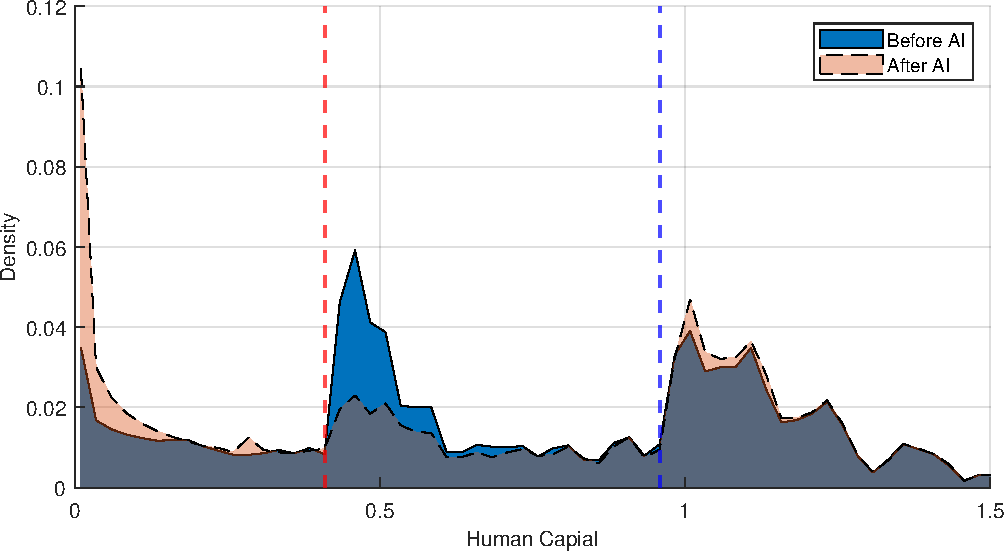
\includegraphics[scale=0.6]{../figure_204040calib/h_dist}
\par\end{center}

\end{frame}

\begin{frame}{Results {\small\textbf{\textit{\textcolor{brown}{~~HC Dynamics}}}}}

\begin{center}
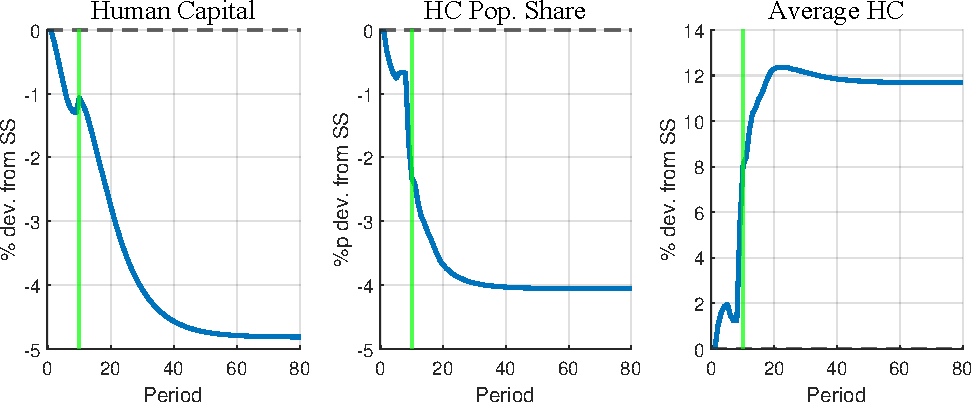
\includegraphics[scale=0.6]{../figure_204040calib/agg_HC}
\par\end{center}

\end{frame}

\begin{frame}{Results {\small\textbf{\textit{\textcolor{brown}{~~Job Polarization}}}}}

\begin{center}
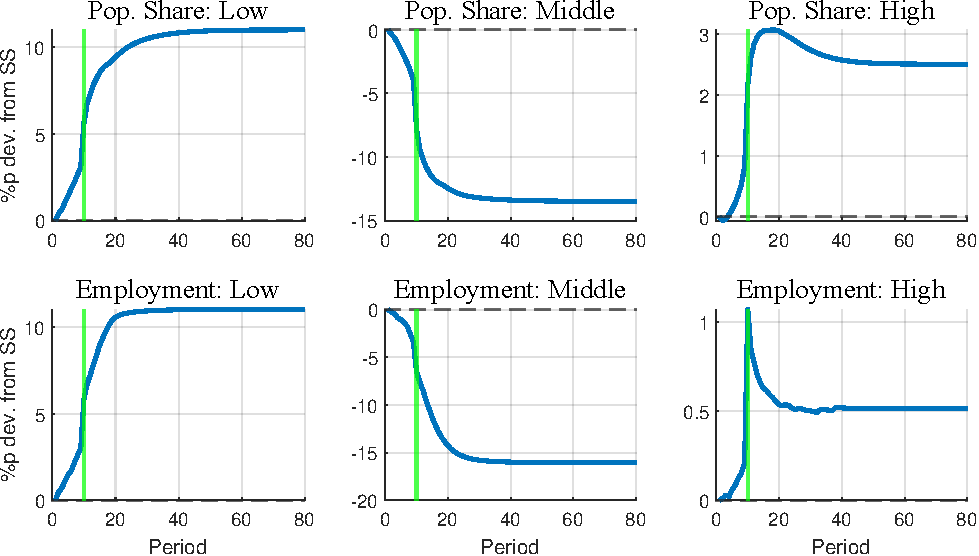
\includegraphics[scale=0.6]{../figure_204040calib/share} 
\par\end{center}

\end{frame}

\begin{frame}{Results {\small\textbf{\textit{\textcolor{brown}{~~Direct and Indirect
Effects}}}}}
\begin{itemize}
\item Effects of AI reflect two forces:
\begin{itemize}
\item \textbf{Direct effect: }AI changes sectoral productivity, shifting
earnings, labor supply, savings, and aggregate output.
\item \textbf{Indirect effect:} Households respond by accumulating human
capital and reallocating across sectors, further affecting productivity
and inequality.

\medskip{}

\end{itemize}
\item To decompose the effect, \textcolor{blue}{we compare the benchmark
model to a No-HC model}
\begin{itemize}
\item The No-HC model captures AI\textquoteright s direct effects, while
the gap identifies the indirect effects. 
\end{itemize}
\end{itemize}
\end{frame}

\begin{frame}{Results {\small\textbf{\textit{\textcolor{brown}{~~Aggregate Effects}}}}}

\begin{center}
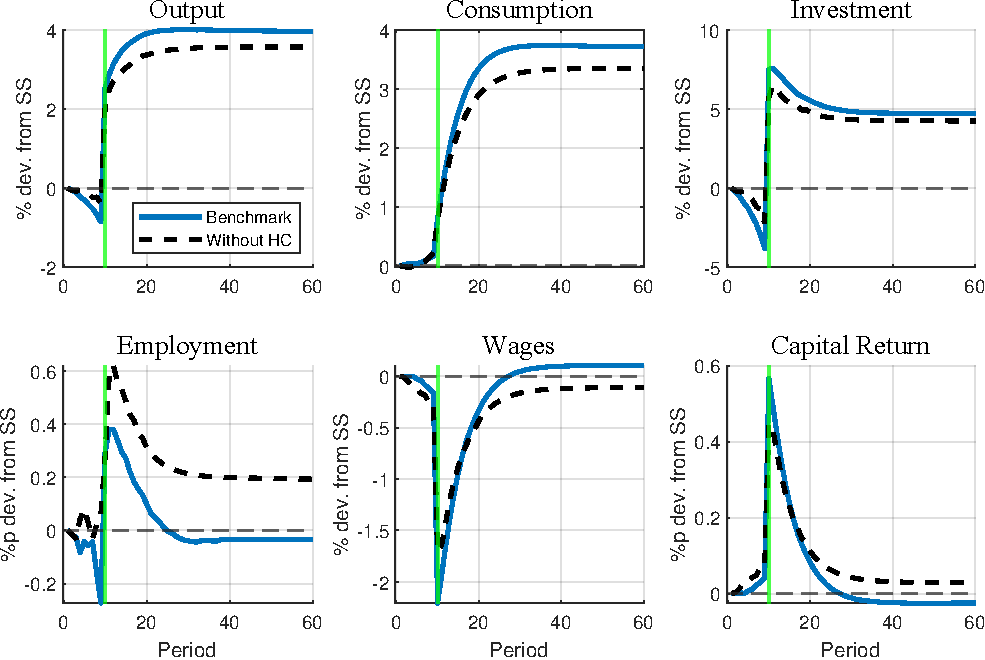
\includegraphics[scale=0.6]{../figure_204040calib/nohc_agg}
\par\end{center}

\end{frame}

\begin{frame}{Results {\small\textbf{\textit{\textcolor{brown}{~~Distributional
Outcomes}}}}}

\begin{center}
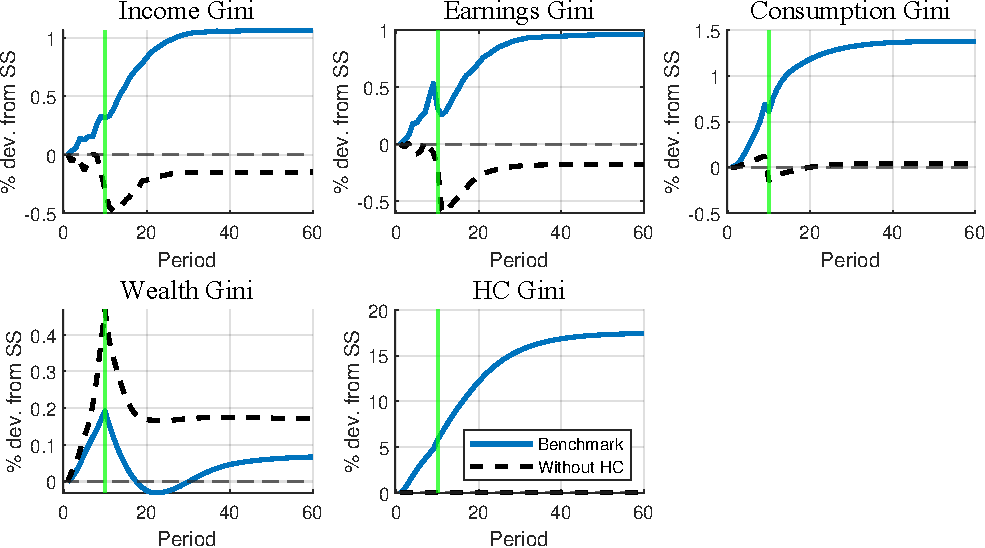
\includegraphics[scale=0.6]{../figure_204040calib/nohc_gini}
\par\end{center}

\end{frame}

\begin{frame}{Results {\small\textbf{\textit{\textcolor{brown}{~~Wealth Inequality}}}}}

\begin{center}
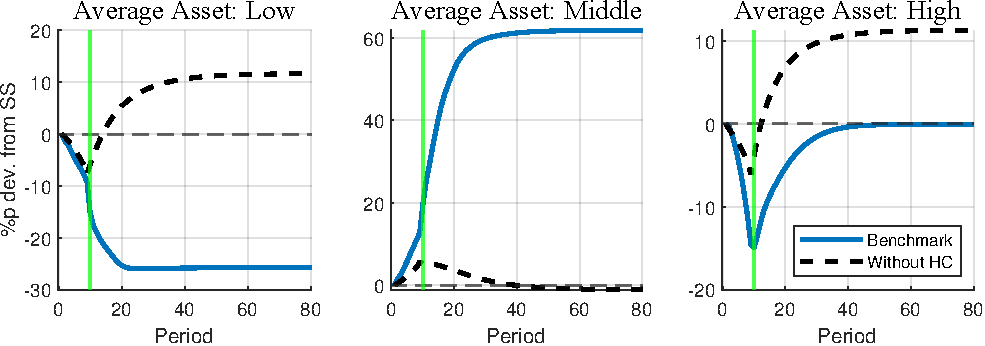
\includegraphics[scale=0.6]{../figure_204040calib/nohc_asset}
\par\end{center}

\medskip{}

\begin{itemize}
\item AI\textquoteright s direct effect: AI affects household saving only
through income effects.
\item Indirect effect from HC: composition channel + \textbf{\textcolor{red}{saving-crowding-in
channel}}
\end{itemize}
\end{frame}

\begin{frame}{AI+ Results {\small\textbf{\textit{\textcolor{brown}{~~High Sector}}}}}

\begin{center}
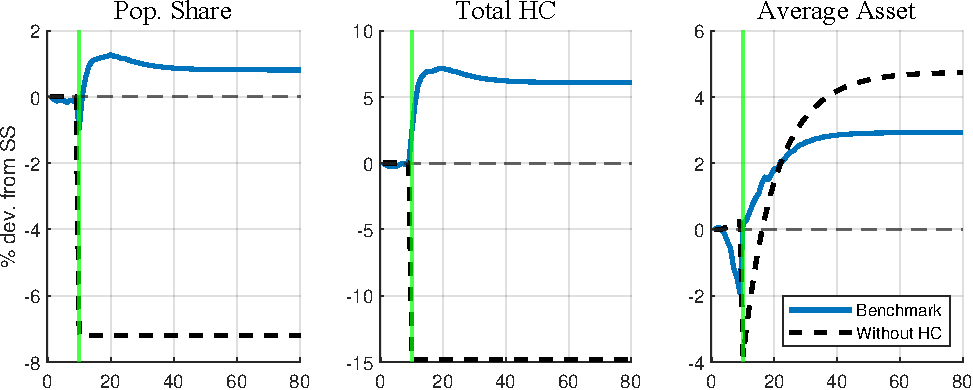
\includegraphics[scale=0.6]{../figure_204040calib/nohc_high_plus}
\par\end{center}

\medskip{}

\begin{itemize}
\item \textbf{Churning effect: }Workers near the new threshold increase
human capital investment to stay in the high sector. 
\end{itemize}
\end{frame}

\begin{frame}{AI+ Results {\small\textbf{\textit{\textcolor{brown}{~~Aggregate
Effects}}}}}

\begin{center}
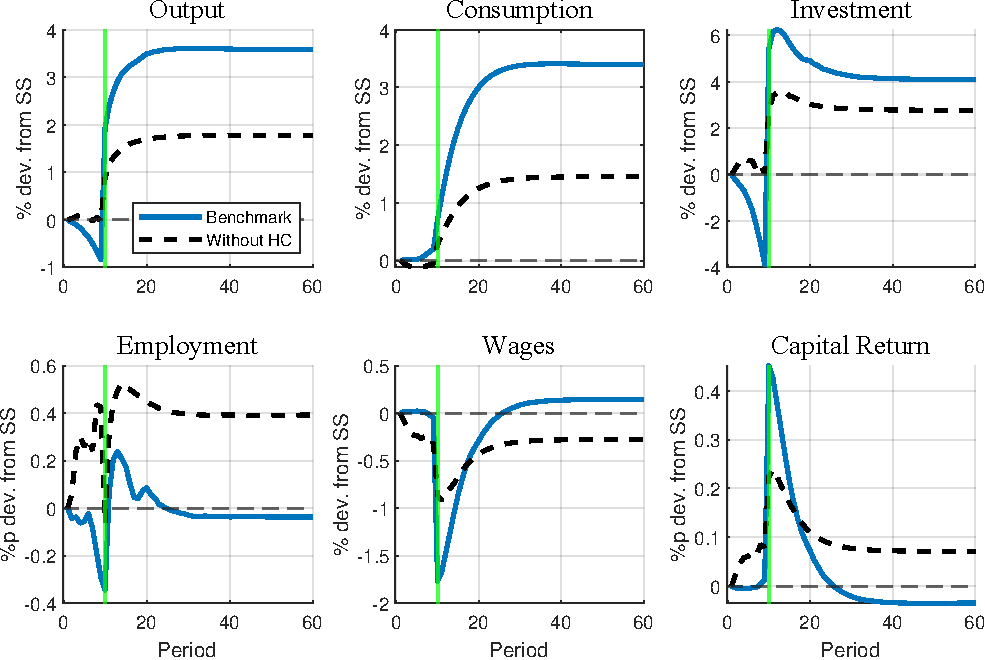
\includegraphics[scale=0.6]{../figure_204040calib/nohc_agg_plus}
\par\end{center}

\end{frame}

\begin{frame}{AI+ Results {\small\textbf{\textit{\textcolor{brown}{~~Distributional
Outcomes}}}}}

\begin{center}
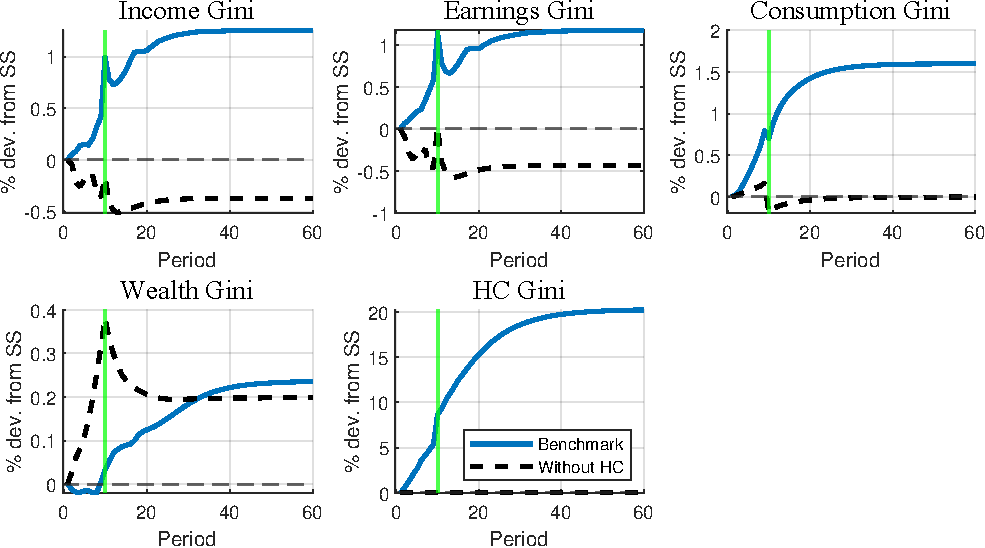
\includegraphics[scale=0.6]{../figure_204040calib/nohc_gini_plus}
\par\end{center}

\end{frame}


\section{Conclusion}
\begin{frame}{Conclusion}

\begin{itemize}
\item \textcolor{black}{This paper analyzes how AI-driven technological
change influences human capital investment and, in turn, affects aggregate
outcomes and economic inequality.}
\item \textcolor{black}{We build an incomplete markets model with endogenous
human capital investment, sectoral structure, transition dynamics,
and general equilibrium feedback.}
\end{itemize}
\bigskip{}

\begin{itemize}
\item \textcolor{black}{The aggregate and distributional effects of AI depend
not only on its direct productivity effects, but also }
\begin{itemize}
\item \textcolor{black}{on households\textquoteright{} anticipatory responses
through retraining; }
\item \textcolor{black}{on its interaction with labor supply adjustment
and precautionary saving.}
\end{itemize}
\end{itemize}
\end{frame}


\end{document}
